\chapter{基于话题演化的改进模型}

\section{引言}

通过上一章的实验结果可以看出,不同的推广策略能够带来不同的推广效果,利用倾向值匹配算法能够在排除混淆变量干扰的情况下,分析推广策略和推广效果之间的因果关系。但是在该实验中,我们仅仅将演员的粉丝量加入到混淆变量当中,即区分了演员不同的流行程度、人气指数对结果的影响。还有其他的众多因素能够影响推广效果,例如演员的性别、年龄、电视剧的演员阵容等,因此需要将更多的因素列入到混淆变量当中进行分析,才能得到更合理更准确的结果。

同时,对于推广周期这一推广模式而言,由于大多数演员会在整个电视剧的宣传周期内持续发布众多的微博,虽然根据倾向值匹配的分析结果,在不同阶段发布的微博能够获得不同的推广效果,但是为达到宣传电视剧的目的,在电视剧上映前中后期都是有必要发布推广微博的。而且随着电视剧所处时间阶段的不同,演员发布推广微博的侧重会有不同,在内容上差异较大,因此,并不应该将微博的推广周期视为一个较为合理的推广模式进行讨论。

考虑到推广周期这一推广模式存在的问题,以及混淆变量数量过少对分析结果造成的影响,我们提出了一种基于话题演化模型的改进方法,对新获取的数据进行了新的实验,更好地对不同的推广模式进行了比较。在改进实验中,将演员发布的推广微博根据话题演化模型分为平稳期和爆发期两组,对于每组内的所有微博分析其推广时间和互动模式这两个推广模式下推广策略的推广效果,并引入演员性别、电视剧评分等更多的混淆变量加入到模型当中,使得分析结果更具有可信性。同时我们还对分析结果进行了模型显著性检验和平衡性检验,验证了倾向值匹配算法的适用性和准确性。

\section{电视剧话题演化规律}

研究发现,微博热点话题在传播过程中,不仅关键词高度集中、受外界环境影响显著,而且传播具有周期性。话题周期一般包括话题发生、话题发展、话题高潮和话题消退四个阶段 \cite{赵龙文2013基于意见领袖参与行为的微博话题热度预测研究}。统计发现,电视剧微博话题演化符合话题演化的基本特征,具有一定的周期特性,如图~\ref{ning}所示,电视剧《柠檬初上》的话题发展正是经历了话题发生、话题发展、话题高潮和话题消退的过程。

\begin{figure}[!htbp]
\centering
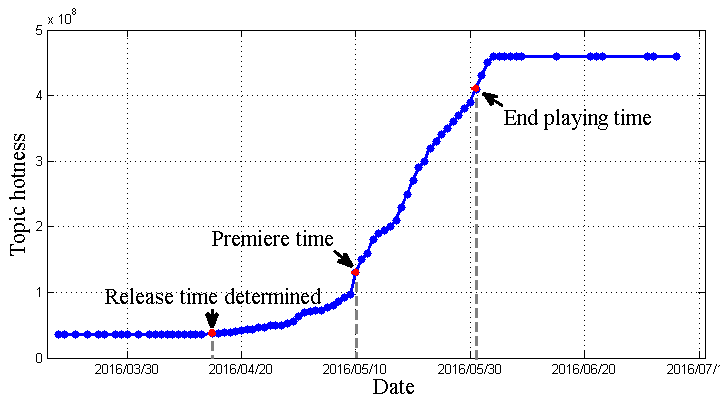
\includegraphics[width=11cm]{2}
\caption{电视剧《柠檬初上》的话题演化过程}
\label{ning}
\end{figure}

在话题演化发展的过程中,“意见领袖”起到了重要的引导作用,他们在信息传播的网络中扮演了关键节点的角色,他们可以为其他人提供信息、传播态度,同时也起到了过滤作用,将其希望传播的信息传递给其他人,而将其不希望传播的信息截留在自身节点处。同样,在电视剧话题演化的过程中,演员就充当了意见领袖的作用,他们不仅拥有很庞大的粉丝群体,还有很大的社交影响力。他们发布的微博信息往往能受到高度关注,在电视剧话题发展过程中,演员发挥了核心作用。在电视剧话题发展过程中有三个重要时间节点导致了电视剧话题向下一阶段的发展,分别是电视剧上映时间确定、首集播出时间、首轮播出结束。在电视剧上映时间确定之前,演员会不时发些电视剧相关信息包括电视剧拍摄进度、拍摄期间趣事、角色定妆照等信息的微博,提前宣传使电视剧话题在微博产生。当电视剧上映时间确定后,主演通常都会发微博宣传电视剧,推动话题发展和酝酿,吸引粉丝和普通用户注意上映时间,吸引第一批群众。当电视剧首轮播放第一集之后,演员发布微博来吸引观看用户参与电视剧剧情、角色相关的讨论,用户也因为看过电视剧,在微博上更愿意参与到话题讨论中去,带来话题热度的大发展。演员和用户的这种行为会持续到电视剧首轮播放结束后几天,之后话题因为其时效性,最终走向消退。

电视剧话题出现期和发展期相对于话题爆发期和消退期存在本质上的差别,即电视剧上映之后,用户对电视剧内容的了解程度和参与程度会发生巨大改变,进而导致话题热度发展不同。因此,本文中将电视剧话题根据电视剧是否上映分成两个主要时期,上映前为平稳期,上映后为爆发期。在电视剧话题的整个发展过程中,因为电视剧所处宣传期不同,演员在微博上的推广方式也会有所差异。例如,对发布推广微博的时间,如图~\ref{time},在平稳期夜晚发布微博很少,白天不同时间发布微博数量比较平稳。但是在爆发期,在电视剧上映前后演员会有一个发布微博的高峰。在此时间发布微博不但能维持既有用户群观看电视剧、参与到电视剧话题讨论,还能吸引和号召新用户观看当天剧情。在不同时期演员发布推广微博的互动模式也有差异,从图~\ref{inter3}可以看出,与平稳期相比,爆发期演员会更多的与官方微博互动。因为当电视剧上映后,官方微博会发布更多的微博,包括剧情讨论、角色讨论、剧照、下集预告等等。

因此,研究演员在不同时期推广策略的有效性是非常有必要的。在本节,我们将演员发布的所有推广微博以电视剧上映的那一天作为时间节点,划分为两个时期分别进行讨论。在各个时期内,利用倾向值匹配算法分析各个推广策略的推广效果。

\section{实验数据}

在本节,为了验证改进模型的可行性和准确性,我们利用新的数据集,从数据库中选取首播时间在2016年1月1日至2016年12月31日之间所有电视剧,以及涉及到的所有演员,一共有313部新的电视剧和对应到微博id的1121位演员,然后从数据库中获取这些演员在这期间发布的所有微博,共114767条微博。最终,演员发布的微博中,只有跟我们研究的电视剧相关的微博被留下作为我们的研究对象,共9185条推广微博。根据3.2.2节介绍的特征提取方法,获得每一条微博的特征向量,如图3.6所示。

\section{推广策略及混淆变量}

与上一章实验相似,我们讨论推广时间和互动模式两个推广模式下的七种推广策略。而推广周期这一模式根据话题演化规律被分为平稳期和爆发期分别进行讨论,对两个时期的微博分别应用倾向值模型,分别评估在两个时期内的有效策略。在倾向值匹配算法中,应该控制混淆变量使得混淆变量在策略组和非策略组分布相似,这样才能更好的分析推广策略的推广效果。考虑到影响一条微博在微博中影响力的因素有很多,除了演员的推广策略本身,还受演员本身属性及电视剧属性等的影响,比如,一个有很多当红演员出演的电视剧可能会比一个几乎没有当红演员出演的电视剧获得更多的关注,造成不同电视剧的推广微博能达到的微博影响力有所差异。因此,本节中我们选用如表~\ref{mul}中包括演员和电视剧相关属性的信息作为混淆变量,使分析结果更具有可靠性。

\begin{table}[!htbp]
\centering
\caption{混淆变量}
\label{mul}
\begin{tabular}{|c|c|} \hline
类别 & 特征\\ \hline
\multirow{3}{*}{演员} & 粉丝数量\\% \hline
& 性别\\% \hline
& 作品数量\\ \hline
\multirow{2}{*}{电视剧} & 演员阵容\\% \hline
&豆瓣评分 \\ \hline
\end{tabular}
\end{table}

同样地,在研究某一项推广策略时,将另一种推广模式下的推广策略归为混淆变量,与以上介绍的这些混淆变量一起加入到混淆变量集合当中进行分析讨论。

\section{数据建模}

对于本实验来说,将倾向值匹配算法应用到实验数据上的方法与上一小节所介绍的实验类似。但由于采用了基于话题演化的模型改进,因此在开始进行分析之前,需要首先将所有微博根据发布的时间,以电视剧的首播时间为分割点,分为平稳期发布的微博和爆发期发布的微博两组,分别进行分析。经过提取和筛选,平稳期共有2569条电视剧相关的推广微博,爆发期共有6616条电视剧相关的推广微博。

同时由于我们在社交网络上提取了更多的信息,也就可以在倾向值匹配模型中加入更多的混淆变量以更好地分析推广策略与推广效果之间的因果关系。之后,根据前文所介绍的方法,应用倾向值匹配算法对这些微博数据进行分析。

首先,对于要分析的每一项推广策略,可以将其他推广模式下的推广策略视为混淆变量。同时,演员的粉丝量也作为混淆变量。将这些混淆变量纳入Logistic回归模型来计算每一条微博的倾向值。

然后,根据是否采用了这项策略,将所有计算出倾向值的微博分为两个样本集合,对两个样本集合中的微博根据其倾向值采用一对多匹配和基于卡尺的最近邻方法进行匹配。在基于卡尺的最近邻匹配过程中,卡尺距离为倾向值对数标准差的$0.2$倍,在我们的数据中卡尺距离为0.09。经过配对,平稳期和爆发期的各个策略下的配对总数如表~\ref{pair}所示。

\begin{table}[!htbp]
\centering
\caption{基于话题演化模型的倾向值匹配结果}
\label{pair}
\begin{tabular}{|c|c|c|c|c|c|} \hline
\multicolumn{2}{|c|}{平稳期}& \multicolumn{2}{c|}{爆发期}\\ \hline
推广策略 & 配对数& 推广策略 & 配对数\\ \hline
早上 & 2423& 早上 & 24699\\% \hline
中午 & 3370 & 中午 & 30163\\% \hline
晚上 & 3049 & 晚上 & 39350\\ \hline
主演互动 & 1226 &  主演互动 & 11756\\
与官微互动& 2435 & 与官微互动 & 8110\\% \hline
原创& 3013 & 原创& 19105\\
其他互动& 3070 & 其他互动 & 29809\\ \hline
\end{tabular}
\end{table}

最后,计算平均干预效果ATT来衡量该项推广策略对推广效果的因果关系。并且,用t检验来检验干预效果的显著性水平,即检验两组微博中的微博影响力水平是否有显著差异。计算标准均数差、画累计分布图和Q-Q图进行平衡性检验。

\section{结果分析}

将倾向值匹配算法分别应用在演员推广的平稳期和爆发期,对各项推广策略进行因果分析,得到的推广策略有效性和t检验结果如表~\ref{res1}所示:

\begin{table}[!htbp]
\centering
\caption{基于话题演化模型的倾向值匹配结果}
\label{res1}
\begin{tabular}{|c|c|c|c|c|c|} \hline
\multicolumn{3}{|c|}{平稳期}& \multicolumn{3}{c|}{爆发期}\\ \hline
推广策略 & ATT & 显著性& 推广策略 & ATT & 显著性\\ \hline
早上 & -0.141 & 0.267& 早上 & 0.222 & 0.410\\% \hline
中午 & 0.023 & 0.837 & 中午 & 0.211 & 0.008\\% \hline
晚上 & 0.359 & 0.024 & 晚上 & -0.176 & 0.004\\ \hline
主演互动 & -0.088 & 0.561 &  主演互动 & -0.078 & 0.302\\
与官微互动& -0.318 & 0.002 & 与官微互动 & -0.001 & 0.989\\% \hline
原创& 2.633 & 0.000 & 原创& 1.860 & 0.000\\
其他互动& -0.743 & 0.000 & 其他互动 & -0.616 & 0.000\\ \hline
\end{tabular}
\end{table}

\textbf{(1)平稳期推广策略效果分析}

从表中可以看出,与在早晨和中午发布微博相比,在晚上发布微博的效果更好。用户晚上通常会花较多的时间在社交网络上,在电视剧上映前,关于电视剧的微博不多,对他们而言,晚上发布的电视剧推广微博有更大的概率被他们看到。对互动模式而言,发布原创微博带来的推广效果要明显远远好于其他互动模式。与之相反,与官微互动和与其他人互动带来的推广效果较差。因为这种微博不能很好的表达演员自己的情感和想法,而且此时电视剧并未上映,粉丝参与电视剧推广微博更多的是因为演员,而不是因为剧情,因此对能更好表达演员自己想法和情感的原创微博会带来更好的粉丝参与度。与此同时,与其他主演互动的模式没有明显好的推广效果。因此在平稳期,晚上发布原创微博会带来最好的推广效果。

\textbf{(2) 爆发期推广策略效果分析}

从表中可以看出,在爆发期,下午发布的推广微博会带来更好的推广效果。虽然微博用户会在晚上花较多时间在社交网络上,但是演员通常在晚上会集中发很多推广微博,导致平均到每条微博的粉丝参与度相对不高。从互动模式来看,发原创微博仍然是最有效的推广策略,原创微博需要演员投入更多的精力编写,同时更好的表达了他的想法和对粉丝参与的期望,而且大部分演员发布的原创微博都是与自身扮演角色相关联,探讨角色性格、命运与自身的看法,粉丝更愿意一起去讨论。而与其他人互动仍然效果最差,与官方微博和其他主演互动的推广效果并不显著。因此可知,在爆发期,演员在下午发布原创微博能获得更好的宣传效果。

\section{模型平衡性检验}

模型平衡性检验的作用是评估倾向值匹配模型是否恰当的进行了应用。对于待验证的各个策略来说,验证模型平衡性包括比较标准均数差和做累计分布图和分位数-分位数图(Q-Q图)。标准均数差验证所有混淆变量在策略组和非策略组的平均值是否有显著差异,作累计分布图和Q-Q图来看混淆变量在策略组和非策略组的分布是否一致。表~\ref{res3}和表~\ref{resmutual}分别显示了两个时期,对于各个时间策略和各个互动策略下,混淆变量的标准偏差。平稳期的标准偏差值在0.001到0.073之间,爆发期的标准偏差值在0.000到0.096之间,表明了策略组和非策略组的匹配样本的平均值分布一致。

\begin{table}[!htbp]
\centering
\caption{推广时间模式下,各个混淆变量的标准偏差}
\label{res3}
\begin{tabular}{|c|c|c|c|c|c|c|} \hline
&\multicolumn{3}{c|}{平稳期}& \multicolumn{3}{c|}{爆发期}\\ \hline
&早上&中午& 晚上 &早上&中午& 晚上\\ \hline
主演互动&0.012&0.073& 0.058&0.028&0.027& 0.008\\ \hline
与官微互动&0.029&0.007& 0.001&0.007&0.011& 0.003 \\ \hline
原创&0.053&0.006& 0.034&0.008&0.003& 0.008\\ \hline
其他互动&0.019&0.009& 0.047&0.018&0.006& 0.006\\ \hline
作品数量&0.006&0.023& 0.007&0.006&0.013& 0.007\\ \hline
性别&0.012&0.003& 0.054&0.023&0.047& 0.010\\ \hline
粉丝数量&0.008&0.033& 0.003&0.005&0.037& 0.002\\ \hline
演员阵容&0.012&0.033& 0.032&0.002&0.023& 0.003\\ \hline
豆瓣评分&0.030&0.049& 0.043&0.002&0.034&0.018\\ \hline
\end{tabular}
\end{table}

\begin{table}[!htbp]
\centering
\caption{互动模式下,各个混淆变量的标准偏差}
\label{resmutual}
\begin{tabular}{|c|c|c|c|c|c|c|c|c|} \hline
&\multicolumn{4}{c|}{平稳期}& \multicolumn{4}{c|}{爆发期}\\ \hline
&主演&官微& 原创 &其他&主演&官微& 原创 &其他\\ \hline
早上&0.043&0.027& 0.016&0.031&0.023& 0.052&0.041& 0.020\\ \hline
中午&0.041&0.008& 0.036&0.018&0.015& 0.038&0.018& 0.002 \\ \hline
晚上&0.015&0.012& 0.023&0.006&0.025& 0.000&0.018& 0.013\\ \hline
作品数量&0.009&0.073& 0.035&0.057&0.014& 0.016&0.017& 0.011\\ \hline
性别&0.046&0.003& 0.035&0.006&0.031& 0.035&0.059& 0.015\\ \hline
粉丝数量&0.025&0.095& 0.014&0.032&0.007& 0.040&0.010& 0.004\\ \hline
演员阵容&0.043&0.096& 0.029&0.035&0.008& 0.041&0.015& 0.004\\ \hline
豆瓣评分&0.036&0.010& 0.024&0.026&0.036&0.025&0.047& 0.014\\ \hline
\end{tabular}
\end{table}

以推广时间模式下的晚上发布推广微博策略和互动模式下的发布原创微博策略为例,如图~\ref{restime}和图~\ref{res2},绘制连续变量:演员粉丝量、作品数、电视剧评分、电视剧阵容的累计分布图和Q-Q图,来刻画策略组和非策略组的混淆变量的分布情况。从图中可以看出,针对这两个策略,平稳期和爆发期的策略组和非策略组的这几个连续混淆变量的分布都非常类似,说明混淆变量得到了控制,分析的推广策略和推广效果之间的因果关系是排除了混淆变量的干扰。因此,倾向值匹配算法在我们的数据中得到了适当的应用,结果准确。

\begin{figure}[h]
  \centering%
  \subcaptionbox{平稳期\\.}
    {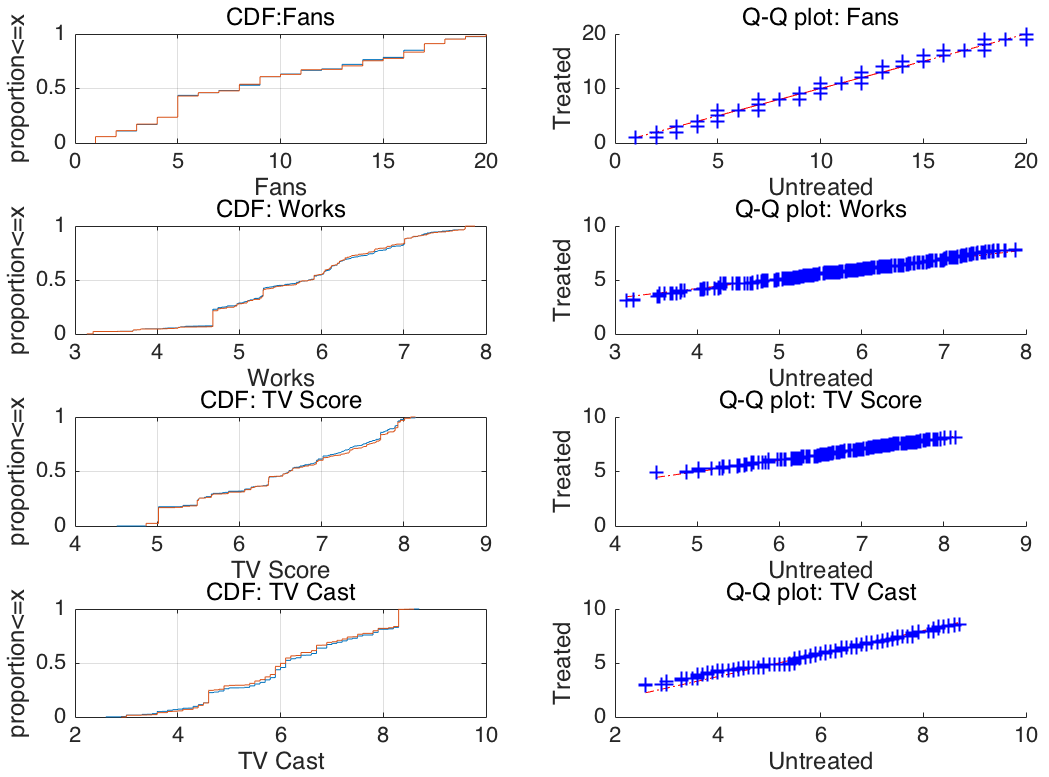
\includegraphics[width=11.5cm,height=11cm]{9}}
  \subcaptionbox{爆发期}
    {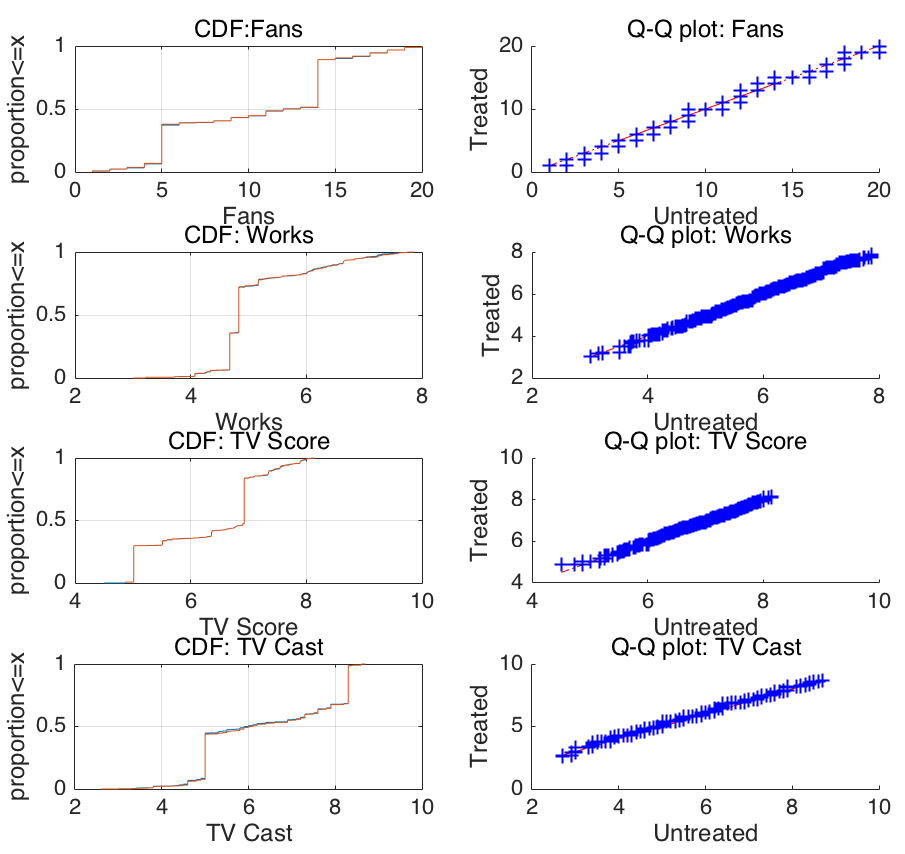
\includegraphics[width=11.5cm,height=10cm]{10}}
\caption{对于晚上发布微博策略的平衡性检验}
\label{restime}
\end{figure}


\begin{figure}[h]
  \centering%
  \subcaptionbox{平稳期\\.}
    {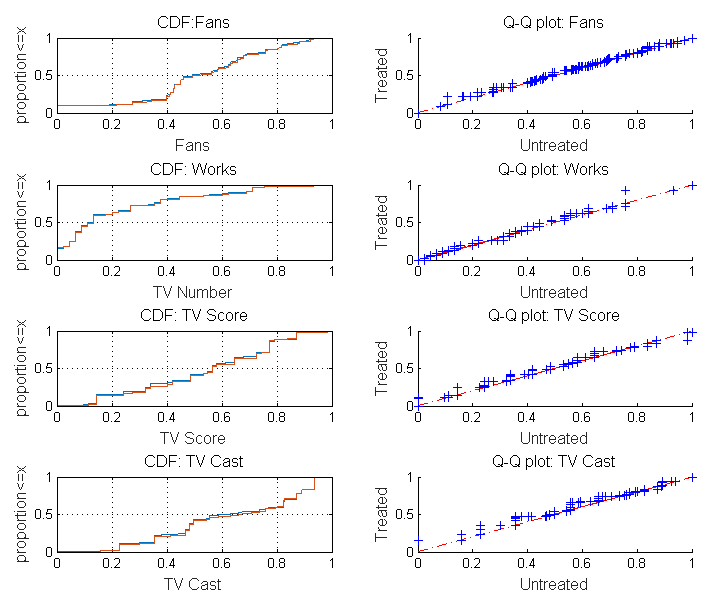
\includegraphics[width=12cm]{7}}
  \subcaptionbox{爆发期}
    {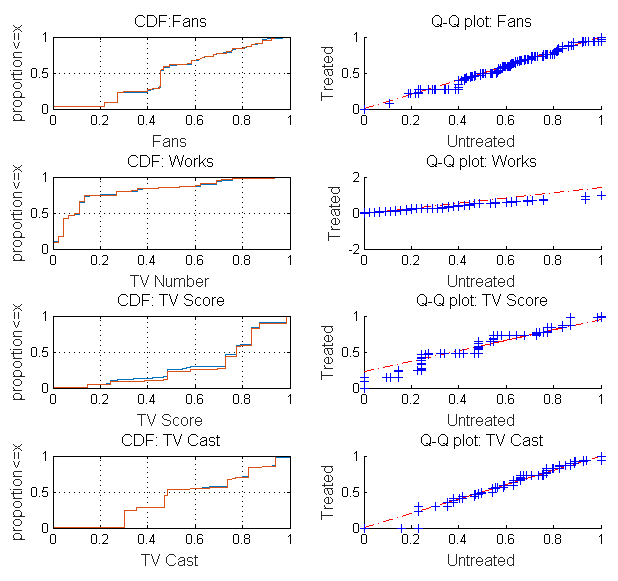
\includegraphics[width=12cm]{8}}
\caption{对于原创微博策略的平衡性检验}
\label{res2}
\end{figure}

\section{本章小结}

本章利用倾向值匹配算法对演员发布的推广微博进行分析时存在的问题,在倾向值匹配算法的基础上,提出了改进的影响力模型。不但结合话题演化规律,将演员的推广行为根据电视剧首播时间,分成两个时间段,而且考虑到各种可能影响推广效果的变量,还加入了更多的混淆变量,使得结果更具有合理性和准确性。而且我们对实验结果进行了显著性分析和平衡性检验,结果显示我们的模型得到了正确、合适的应用。



































